% Define document class
\documentclass[twocolumn]{aastex63}
\DeclareRobustCommand{\Eqref}[1]{Eq.~\ref{#1}}
\DeclareRobustCommand{\Figref}[1]{Fig.~\ref{#1}}
\DeclareRobustCommand{\Tabref}[1]{Tab.~\ref{#1}}
\DeclareRobustCommand{\Secref}[1]{Sec.~\ref{#1}}
\newcommand{\todo}[1]{{\large $\blacksquare$~\textbf{\color{red}[#1]}}~$\blacksquare$}
\newcommand{\mr}[1]{{\textbf{\color{green!75!black}[#1]}}}
% \usepackage{cuted}
\usepackage{flushend}
\usepackage{amsmath}
% \graphicspath{{./figures/}}

\begin{document}

% Title
\title{On the prevalence of early mass transfer for very massive binaries}

\author[0009-0008-2061-4946]{C.~A.~Burt}
\affiliation{University of Arizona, Department of Astronomy \& Steward Observatory, 933 N.~Cherry Ave., Tucson, AZ 85721, USA}

\author[0000-0002-6718-9472]{M.~Renzo}
\affiliation{University of Arizona, Department of Astronomy \& Steward Observatory, 933 N.~Cherry Ave., Tucson, AZ 85721, USA}

\author[0000-0002-2215-1841]{A.~Grichener}
\affiliation{University of Arizona, Department of Astronomy \& Steward Observatory, 933 N.~Cherry Ave., Tucson, AZ 85721, USA}

\author{\todo{TBD}}

\begin{abstract}
  Common phases of mass transfer in stellar binaries are case A
  (during the donor's main sequence) and case B (after the donor's
  main sequence but before helium core depletion). Typically, stellar
  radii significantly grow after the main sequence, making case B more
  common. However, very massive stars may already undergo significant
  expansion during the main sequence increasing the probability of
  case A mass transfer.  For observationally-informed convective
  boundary mixing, case A dominates for donor masses
  $\gtrsim 75 \, M_{\odot}$. This is not the case without convective
  boundary mixing or in the stellar models commonly used in rapid
  binary population synthesis.  Therefore, case A mass transfer may be
  more dominant than commonly assumed, with potential impact on rates
  of all post mass transfer binaries, from Wolf-rayet-O-type binaries,
  to X-ray binaries, and gravitational wave progenitors.
\end{abstract}

\section{Mass Transfer in Very Massive Binaries}

Binary stars with a sufficiently small orbital separation
($a\lesssim2500\,R_{\odot}$) undergo (at least) a mass transfer phase
in which the donor star transfers mass to the initially less massive
accretor [CITE?]. For very massive stars ($ \gtrsim 30 \, M_{\odot}$), mass
transfer most often occurs during the donor's hydrogen core-burning
(case A) or helium core-burning (case B), which together cover
$\sim99\%$ of the donor's lifetime \citep{kippenhahn:67}.

\begin{figure*}[htbp]
  \centering
  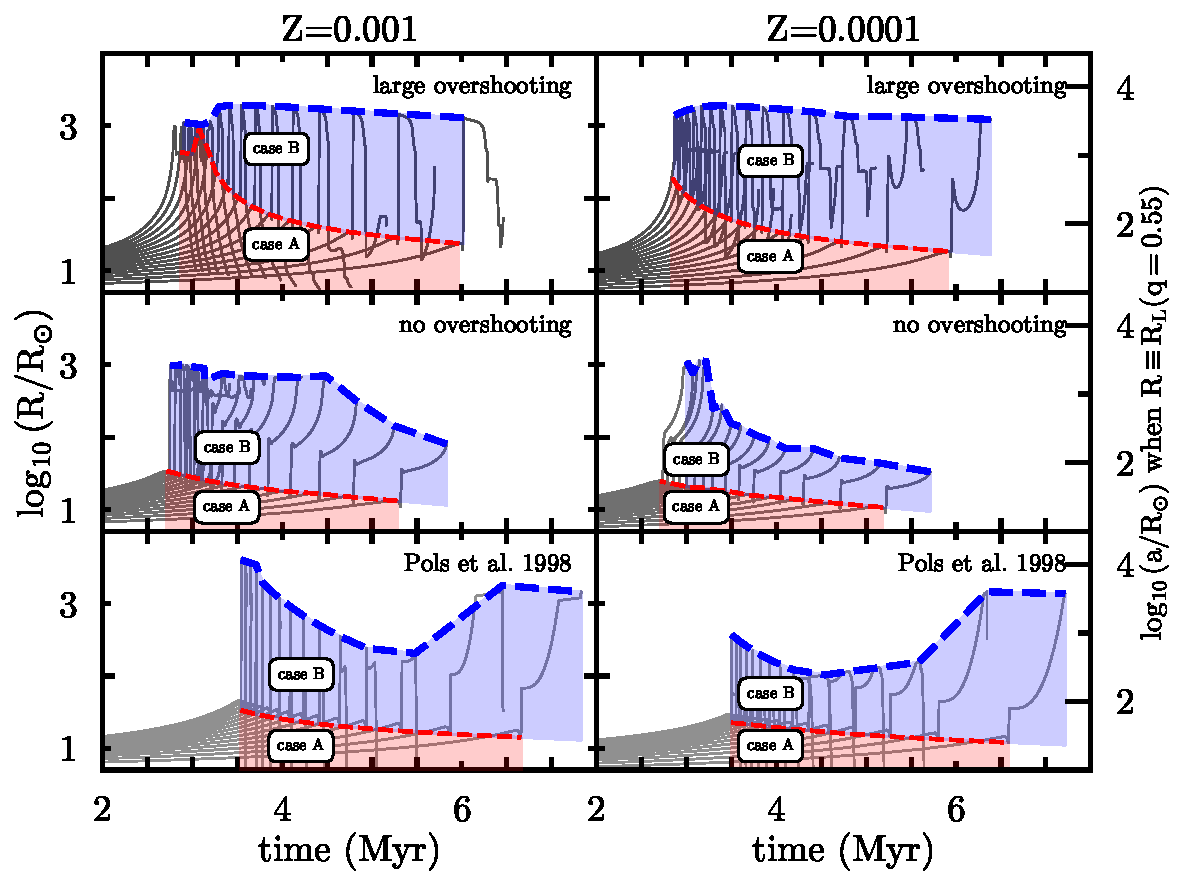
\includegraphics[width=0.9\textwidth]{radii}
  \caption{Each panel contain 15 stellar \textsc{MESA} models spanning
    from $30 \, M_{\odot}$ star (longer lifetimes) to
    $100 \, M_{\odot}$ (shorter lifetimes). The top panels show
    models with \cite{brott:11}-like convective boundary mixing (``large'' overshooting), the
    middle show models without overshooting, and the bottom panels
    plot models generated from \textsc{COMPAS} based on analytic fits
    to the stellar models of \cite{pols:98}. The left (right) panels
    have a metallicity $Z=0.001$ ($Z=0.0001$). Dashed red (blue) lines
    mark the maximum radius during the main sequence (during the runtime of the model). The red (blue) shaded areas underneath correspond to
    case A (case B) mass transfer.}
  \label{fig:radii}
\end{figure*}


For a flat in $\log_{10}(a)$ initial separation distribution
\citep{opik:24}, case B is expected more often than case A mass
transfer, since most stars expand dramatically post-main sequence
\citep{vandenheuvel:69}. However, very massive stars may already
undergo a drastic expansion in radius during their main sequence.
\citep[e.g.,][]{sanyal:15, jiang:15, sabhahit:24}. This may increase
the rate of case A, affecting the evolution of the star and
consequently potentially altering stellar parameters that determine
the rate of Wolf-Rayet+O-type binaries \citep[e.g.,][]{nuijten:24},
X-ray binaries, and gravitational wave progenitors.

The radius of the
donor is dependent on unknown stellar parameters, including stellar
winds \citep{renzo:17, josiek:24}, metallicity \citep{xin:22},
close-to-super-Eddington-layers \citep[e.g.,][]{joss:73, paxton:13,
  jiang:15, agrawal:22, jermyn:23}, and convective boundary mixing
\citep{anders:23, johnston:24}. Here, we illustrate this comparing the
radial evolution of very massive stars while varying convective boundary
mixing and metallicity with models commonly adopted in rapid binary
population synthesis.

\section{Comparing Donor Radii}

We computed \textsc{MESA} models\footnote{Publicly available at
  \href{https://doi.org/10.5281/zenodo.14757819}{doi.org/10.5281/zenodo.14757819}} (version 24.03.1,
\citealt{paxton:11, paxton:13, paxton:15, paxton:18, paxton:19,
  jermyn:23}) from $30 \, M_{\odot}$ to $100 \, M_{\odot}$ in steps of
$5\,M_\odot$ at metallicity $Z=0.001$ and $0.0001$ following the setup
from \cite{renzo:23}. The gray lines in \Figref{fig:radii} show their
radial evolution as a function of time.

We explore models with (top panel) and without overshooting (middle
panel) and compare them to the \cite{pols:98} models (bottom panel)
used in \textsc{SSE} \citep{hurley:00} generated using \textsc{COMPAS}
\citep{stevenson:17, vignagomez:18, riley:22}, which extrapolates for
masses $\geq50\,M_\odot$.

When using overshooting, our \textsc{MESA} models implement an
exponential algorithm \citep{herwig:00} fit to the step overshooting
calibrated on the width of main sequence in 30 Doradus
\citep{brott:11} following \cite{claret:18}. This relatively ``large
overshooting'' model is compared to models not including any
convective boundary mixing, and to the \cite{pols:98} models including
an effectively mass-dependent overshooting.

The red and blue dashed lines in each panel of \Figref{fig:radii}
denote the maximum radius during the main sequence and helium core
burning phase, respectively. These mark the maximum Roche radius for a
case A and case B donor, respectively. The right axis shows orbital
separations $a$ where the stellar radius meets the roche radius
\citep{eggleton:83}, assuming a representative accretor-to-donor mass
ratio of $q=0.55$, corresponding to the average for a flat mass-ratio
distribution between 0.1 and 1 \citep{kobulnicky:07,sana:12}. The red regions
denote binaries which will undergo case A mass transfer and the blue
regions denote binaries which will undergo case B mass transfer.

For $Z=0.001$, when including overshooting (top left panel), donors
with masses $ \gtrsim 75 \, M_{\odot}$ can only experience case A.
Removing convective boundary mixing (middle) keeps main sequence radii
smaller, preserving the blue region above the red line for case B mass
transfer at all masses. The overshooting implementation from
\cite{pols:98} (bottom), while nonzero, still leaves a large window
for case B up to at least $100 \, M_{\odot}$. At even lower
metallicities of $Z=0.0001$ (right), stars are more compact, and all
models allow for case B mass transfer at all masses.

\section{Implications for Post-Mass-Transfer Binaries}

Convective boundary mixing \citep{brott:11, johnston:24} and
metallicity have a strong effect on stellar radii, which determine
when a donor fills its Roche lobe. Related effects on stellar radii have
been explored elsewhere, including the adopted wind mass loss rates
\citep[e.g.,][]{smith:14, renzo:17, josiek:24}, rotation (and
consequently tides, e.g., \citealt{maeder:00}), and the treatment of energy transport
in correspondende of opacity bumps in the envelope
\citep[e.g.,][]{joss:73, agrawal:22, cheng:24}.

After a thermal-timescale initial phase, Case A mass transfer occurs
overall on a longer (nuclear) timescale, while case B occurs entirely
on a much shorter (thermal) timescale \citep[but see][]{klencki:22}.
Moreover, the dynamical stability of the orbit during mass transfer is
sensitive to the evolutionary phase of the stars involved
\citep[e.g.,][]{claeys:14}. Therefore, whether a given binary
experiences a common envelope evolution,which is critical to determine
the outcome of the binary system, depends on more than just the mass
ratio, as generally assumed in rapid population synthesis. Comparing
rows in \Figref{fig:radii} shows that the stellar evolution models
commonly used in rapid population synthesis are qualitatively similar
to our no overshooting models, in the sense that they allow for case B
mass transfer in all mass regions we sampled and for metallicities
relevant to galactic and gravitational astronomy.

Given the critical role of mass transfer for the formation of many
binaries of interest, the fraction of systems experiencing case A in
respect to case B may significany impact predicted rates for post mass
transfer binaries, including Wolf-Rayet+O-type binaries, X-ray
generated usingbinaries, and gravitational wave progenitors. In
particular, the role of the stable mass transfer channel
\citep[e.g.,][]{marchant:21, vanson:22} for (massive) binary black
hole mergers is currently hotly debated. Our results highlight that
stellar uncertainties influence the mode of mass transfer and
consequently the outcomes.


\software{This work made use of the following software packages:
  \texttt{matplotlib} \citep{Hunter:2007} and \texttt{python}
  \citep{python}, \url{http://github.com/TeamCOMPAS/COMPAS}, and
  \url{https://docs.mesastar.org} MESA. Software citation information
  aggregated using
  \texttt{\href{https://www.tomwagg.com/software-citation-station/}{The
      Software Citation Station}}
  \citep{software-citation-station-paper,
    software-citation-station-zenodo}.}

\bibliography{./donorR.bib}
\end{document}

%%% Local Variables:
%%% mode: LaTeX
%%% TeX-master: t
%%% End:
